\documentclass[border=10pt]{standalone}
\usepackage[svgnames]{xcolor}
\usepackage{amsmath}
\usepackage{pgfplots}
\pgfplotsset{compat=newest}
\usepackage[sfdefault]{FiraSans}
\usepackage{FiraMono}
\renewcommand*\familydefault{\sfdefault}
\begin{document}
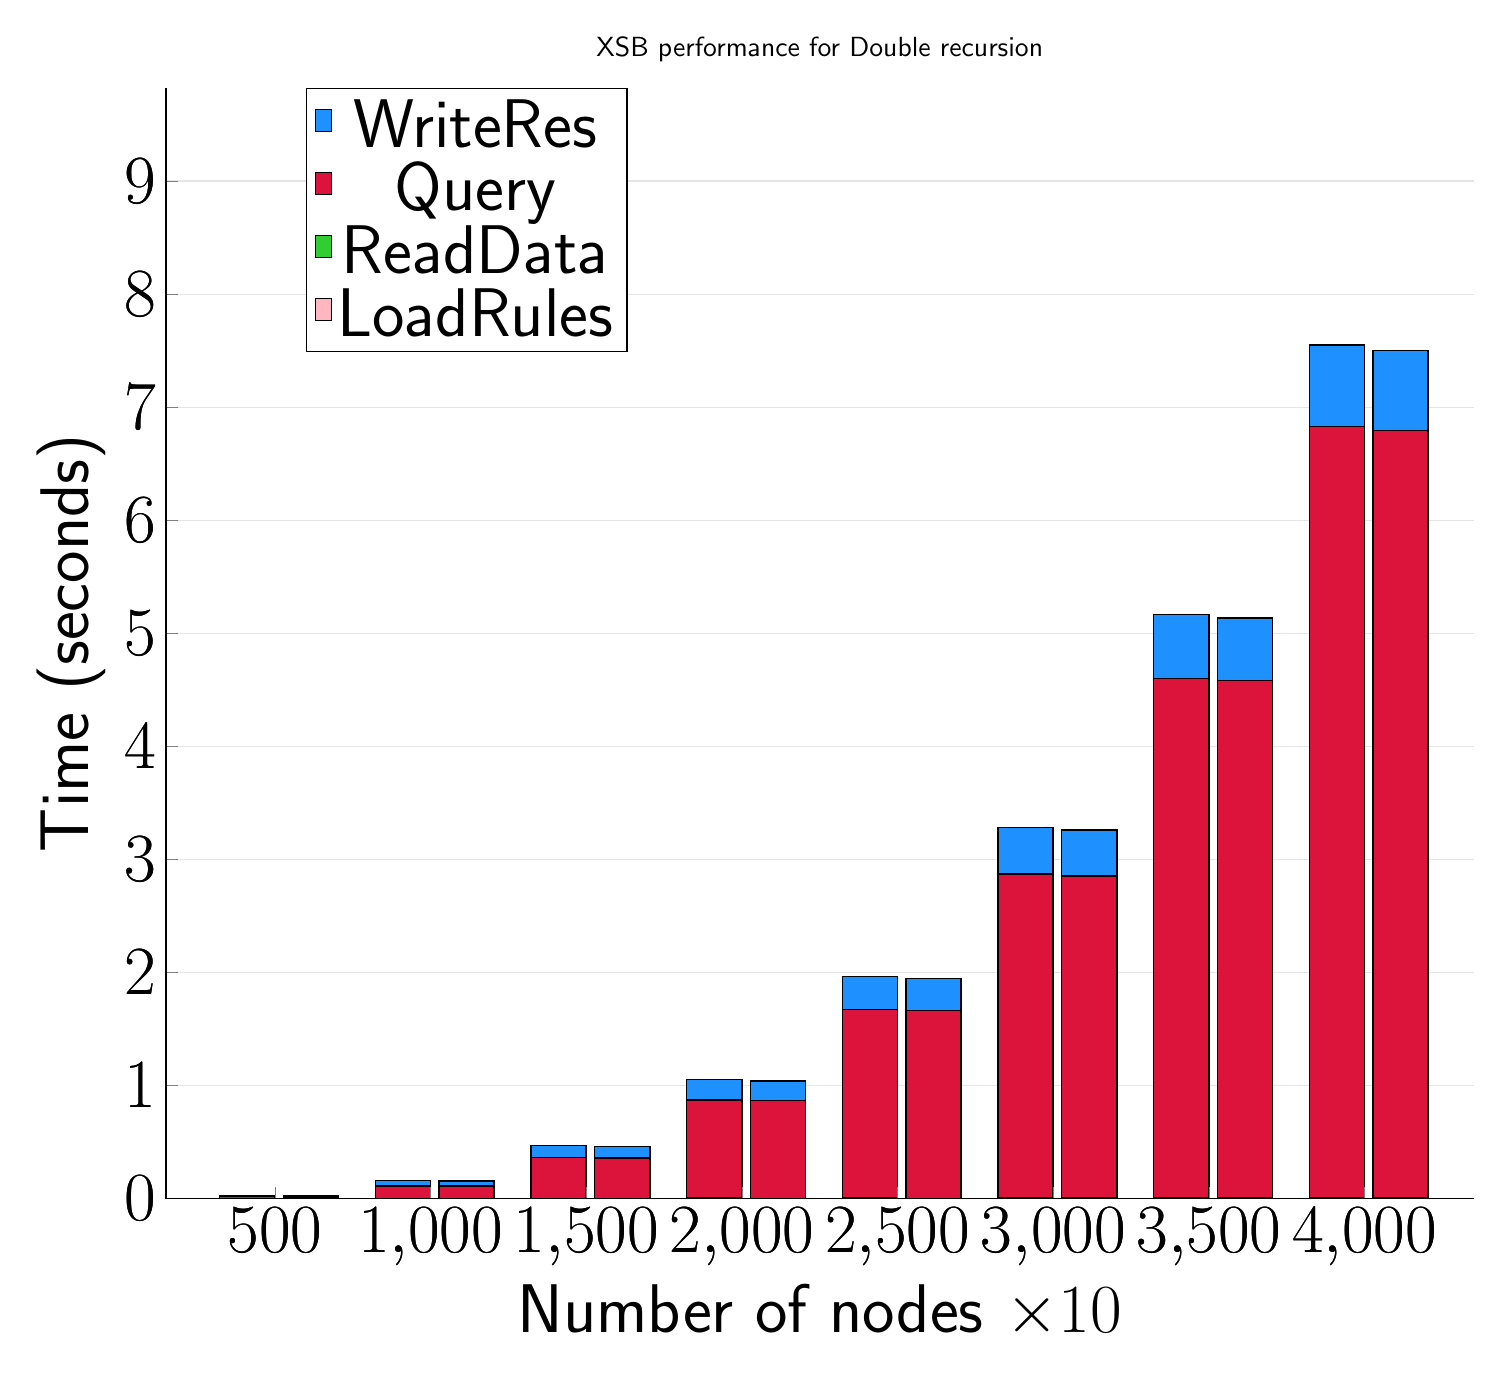
\begin{tikzpicture}
	\begin{axis}[
			ybar stacked,
			title={XSB performance for Double recursion},
			bar shift=-10pt,
			width=1.5\textwidth,
			bar width=0.7cm,
			ymajorgrids, tick align=inside,
			major grid style={draw=gray!20},
			xtick=data,
			ymin=0, ymax=9.824258804321289,
			axis x line*=bottom,
			axis y line*=left,
			enlarge x limits=0.1,
			legend style={
					at={(0.23, 1)},
					anchor=north,
					legend columns=1,
					font=\Huge,
				},
			ylabel={Time (seconds)},
			xlabel={Number of nodes $\times 10$},
			label style={font=\Huge},
			tick label style={font=\Huge},
		]
		\addlegendimage{fill=DodgerBlue, draw=black, line width=0.2pt}
		\addlegendentry{WriteRes}
		\addlegendimage{fill=Crimson, draw=black, line width=0.2pt}
		\addlegendentry{Query}
		\addlegendimage{fill=LimeGreen, draw=black, line width=0.2pt}
		\addlegendentry{ReadData}
		\addlegendimage{fill=LightPink, draw=black, line width=0.2pt}
		\addlegendentry{LoadRules}
		\addplot +[fill=LightPink, draw=black, line width=0.5pt] coordinates {
				(500, 0.0010653972625732431)
				(1000, 0.0010470867156982418)
				(1500, 0.001035714149475099)
				(2000, 0.0010777235031127921)
				(2500, 0.001107025146484376)
				(3000, 0.0010823011398315432)
				(3500, 0.0012523651123046882)
				(4000, 0.00137615203857422)
			};
		\addplot +[fill=LimeGreen, draw=black, line width=0.5pt] coordinates {
				(500, 0.0007867097854614257)
				(1000, 0.001278495788574218)
				(1500, 0.001796698570251464)
				(2000, 0.002310991287231445)
				(2500, 0.002795863151550293)
				(3000, 0.003264904022216799)
				(3500, 0.003801918029785155)
				(4000, 0.004217767715454101)
			};
		\addplot +[fill=Crimson, draw=black, line width=0.5pt] coordinates {
				(500, 0.014225888252258312)
				(1000, 0.11008560657501239)
				(1500, 0.36039953231811533)
				(2000, 0.8680027008056641)
				(2500, 1.669307327270507)
				(3000, 2.865211462974547)
				(3500, 4.597123241424562)
				(4000, 6.824258804321289)
			};
		\addplot +[fill=DodgerBlue, draw=black, line width=0.5pt] coordinates {
				(500, 0.01173932552337645)
				(1000, 0.04578676223754859)
				(1500, 0.10377321243286122)
				(2000, 0.1813956975936879)
				(2500, 0.290834259986877)
				(3000, 0.4138795614242571)
				(3500, 0.5656513690948459)
				(4000, 0.720202922821044)
			};
	\end{axis}
	\begin{axis}[
			ybar stacked,
			bar shift=13pt,
			width=1.5\textwidth,
			bar width=0.7cm,
			ymajorgrids, tick align=inside,
			major grid style={draw=none},
			xtick=data,
			ymin=0, ymax=9.824258804321289,
			axis x line*=none,
			axis y line*=none,
			enlarge x limits=0.1,
			label style={font=\Huge},
			tick label style={font=\Huge},
		]
		\addplot +[fill=LightPink, draw=black, line width=0.5pt] coordinates {
				(500, 0.0006186000000000002)
				(1000, 0.0006103)
				(1500, 0.0006009000000000003)
				(2000, 0.0006256999999999999)
				(2500, 0.0006299000000000001)
				(3000, 0.0006182999999999998)
				(3500, 0.0006496999999999998)
				(4000, 0.0006337000000000003)
			};
		\addplot +[fill=LimeGreen, draw=black, line width=0.5pt] coordinates {
				(500, 0.0005550999999999996)
				(1000, 0.0010019)
				(1500, 0.0014396)
				(2000, 0.0019598000000000003)
				(2500, 0.0024005000000000003)
				(3000, 0.0028473000000000005)
				(3500, 0.0033237)
				(4000, 0.0037085)
			};
		\addplot +[fill=Crimson, draw=black, line width=0.5pt] coordinates {
				(500, 0.014000199999999999)
				(1000, 0.1090539)
				(1500, 0.3579511000000001)
				(2000, 0.8624541000000001)
				(2500, 1.6583755999999998)
				(3000, 2.8507938)
				(3500, 4.575917)
				(4000, 6.790781300000001)
			};
		\addplot +[fill=DodgerBlue, draw=black, line width=0.5pt] coordinates {
				(500, 0.011263200000000001)
				(1000, 0.0447244)
				(1500, 0.10171960000000002)
				(2000, 0.1764765)
				(2500, 0.28683500000000006)
				(3000, 0.40619570000000016)
				(3500, 0.5543880999999999)
				(4000, 0.7079360999999997)
			};
	\end{axis}
\end{tikzpicture}

\end{document}
